\chapter{Introduction}
\label{chap-introduction}

Beginning in 2004, computer scientists from Harvard University joined forces
with seismologists from the University of New Hampshire, the University of
North Carolina, and Instituto Geof\'{i}sico, Escuela Polit\'{e}cnica Nacional,
Ecuador, to begin a collaboration aimed at using sensor networks to further the
study of active volcanoes. As of early 2009 our collaboration has spanned
three successful deployments, multiple scientific publications and generated a
large number of interesting ideas to explore.  We have been fortunate to be a
part of this long-running partnership.

From a simple starting point --- a handful of nodes streaming continuous data
from a single sensor per node --- we have developed a sophisticated
resource-aware architecture carefully balancing the value of the data to the
application against the network-wide cost of extraction. These design changes
were motivated by the science goals, responsive to changing hardware
platforms, and driven by experience gained deploying prior iterations.
Because each of the three deployments is already well-documented, one of
our goals is to illuminate the design process by linking successive artifacts
together while maintaining the thread of data quality as an application
driver.

From the beginning of our work, providing high quality data has remained a
part of our research agenda. This focus emerged out of both the scientific
goals, and constraints of the devices we have deployed. Because seismologists
are used to processing high-resolution data from multiple stations, wireless
sensor networks --- while considerable less burdensome than existing
instrumentation --- must provide data of similar quality before they can be
used for scientific study.  The scale made possible by rapid deployment
promised by augmenting existing seismological instrumentation with wireless
sensor network hardware is new, but the existence of data processing
techniques means that the requirements are already firmly in place.

Designing wireless sensor network applications in this space has required work
to meet some of the data quality requirements while finding ways of creatively
relaxing others.  Specifically, we have found it necessary to deliver
high-resolution data meeting strict timing requirements, but found flexibility
in terms of providing a complete data set from every node covering all moments
of time.

\section{Overview of Seismoacoustic Monitoring}

Volcanic monitoring has a wide range of goals, related to both scientific
studies and hazard monitoring. Figure~\ref{fig-cartoon} displays an overview
of several instruments that might be used, the signals that they collect and
example configurations used during deployments. The type and configuration of
the instrumentation depends on the goals of a particular study.
Traditionally, dispersed networks of seismographs, which record
ground-propagating elastic energy, are utilized to locate, determine the size
of, and assess focal mechanisms (source motions) of earthquakes occurring
within a volcanic edifice~\cite{Chouet03}.  At least four
spatially-distributed seismographs are required to constrain hypocentral (3D)
source location and origin time of an earthquake, though using more seismic
elements enhances hypocenter resolution and the understanding of source
mechanisms. Understanding spatial and temporal changes in the character of
volcanic earthquakes is essential for tracking volcanic activity, as well as
predicting eruptions and paroxysmal events~\cite{McNutt96}. 

Another use of seismic networks is the imaging of the internal structure of a
volcano through tomographic inversion.  Earthquakes recorded by
spatially-distributed seismometers provide information about propagation
velocities between a particular source and receiver.  A seismically-active
volcano thus allows for three-dimensional imaging of the volcano's velocity
structure~\cite{Benz96,Phillips91}. The velocity structure can then be
related to material properties of the volcano, which may be used to determine
the existence of a magma chamber~\cite{Lees89,Moran99}.  Dense array
configurations, with as many as several dozen seismographs, are also an
important focus of volcanic research~\cite{Dietel89,Neuberg94}. Correlated
seismic body and surface wave phases can be tracked as they cross the array
elements, enabling particle motion and wavefield analysis, source
back-azimuth calculations, and enhanced signal-to-noise recovery.

\section{Opportunities for Wireless Sensor Networks}

\begin{figure}[t] 
\begin{center} 
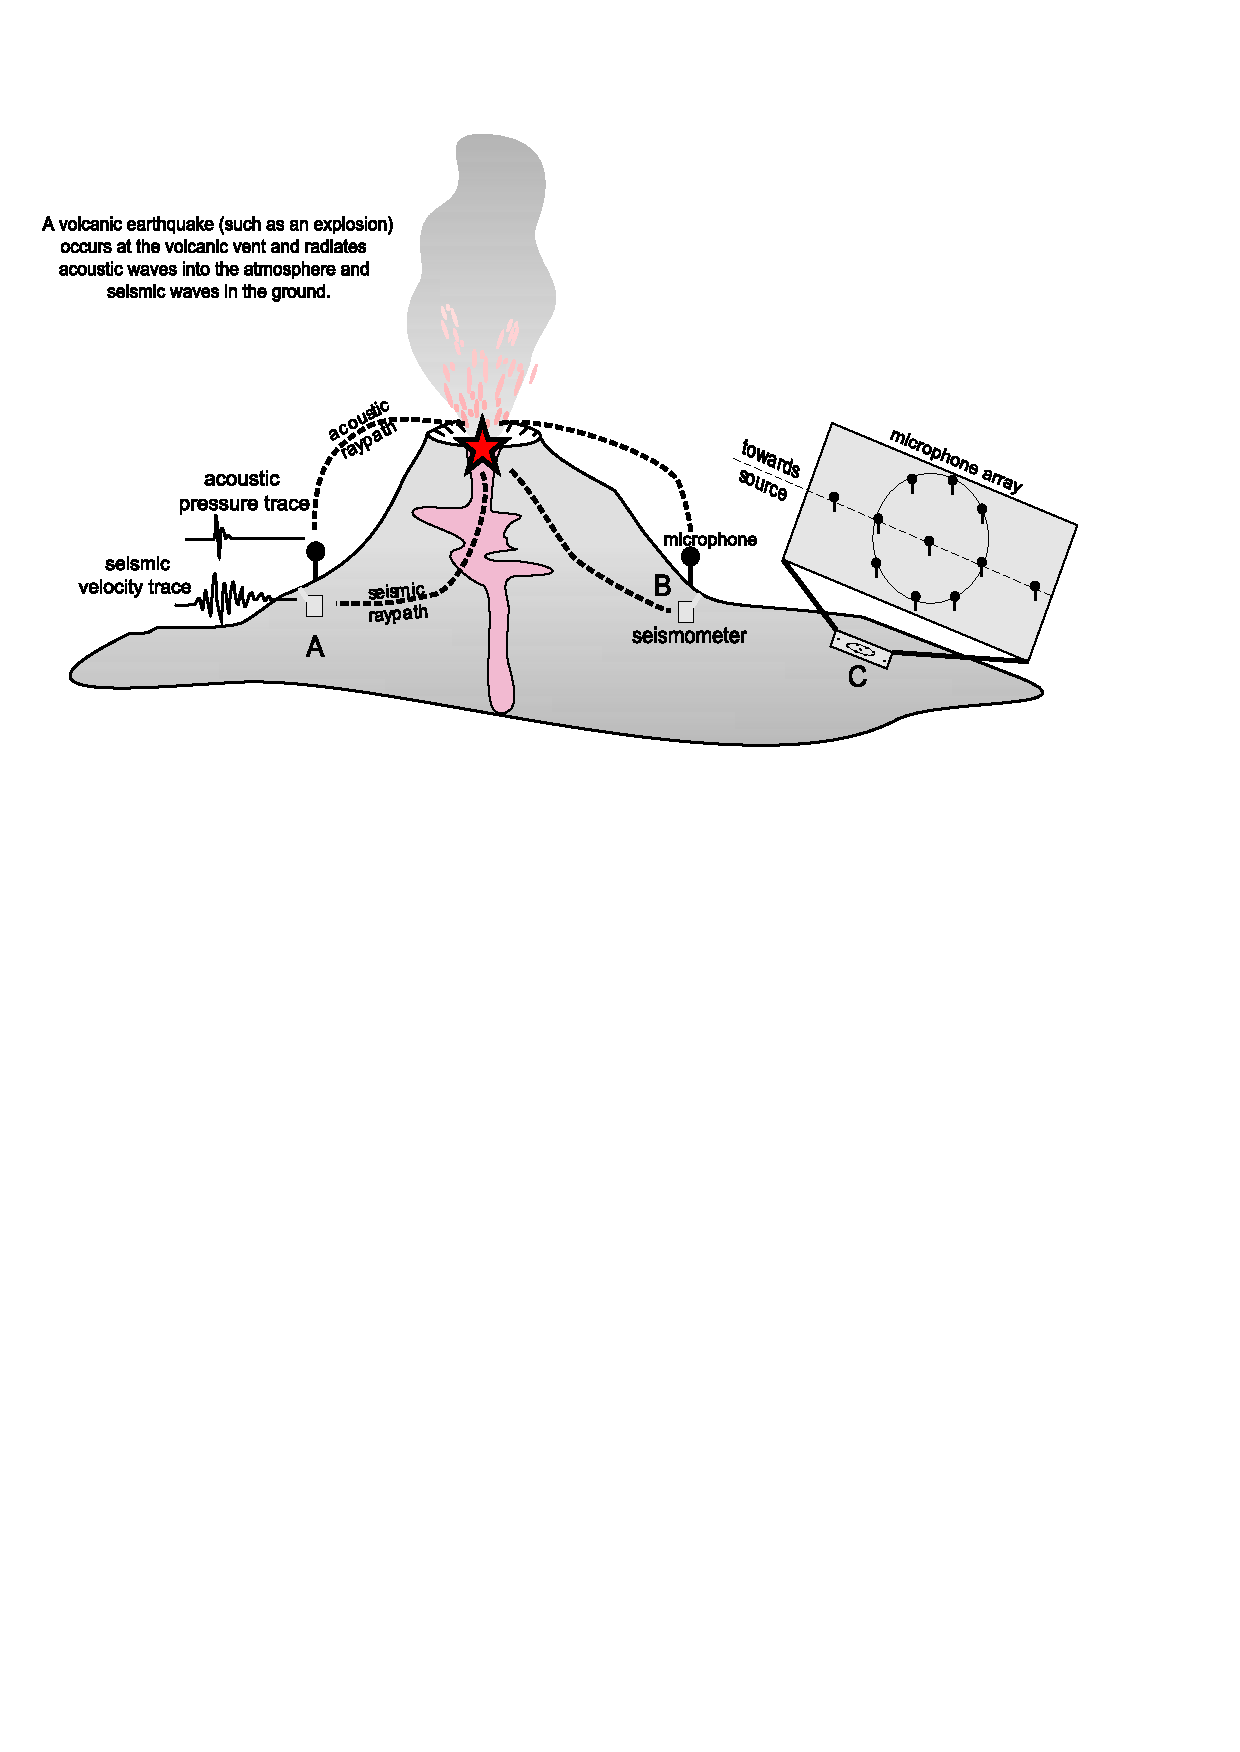
\includegraphics[width=0.9\hsize,clip=true,bb=20 470 540 770]{./resources/EWSN2005/figures/Cartoon2.pdf}
\end{center} 
\caption{{\bf Sensor arrays for volcanic monitoring.}} 
\label{fig-cartoon} 
\end{figure}

Networks of spatially-distributed sensors are commonly used to monitor
volcanic activity, both for hazard monitoring and scientific
research~\cite{Scarpa96}.  Typical types of sensing instruments include
seismic, acoustic, GPS, tilt-meter, optical thermal, and gas flux.  Volcanic
sensors range from widely dispersed instrument networks to more confined
sensor arrays. An individual sensor station could consist of a single sensor
(e.g., seismometer or tilt sensor), or an array of several closely-spaced
($10^2$ to $10^3$~m aperture) wired sensors, perhaps of different types.
Multiple stations may be integrated into a larger network installed over an
extended azimuthal distribution and radial distance ($10^2$ to $10^4$~m) from
the volcanic vent.  Data from various stations may be either recorded
continuously or as triggered events and the acquisition bandwidth depends
upon the specific data stream. For instance, seismic data is often acquired
at 24-bit resolution at 100~Hz, while tilt data may be recorded with 12-bit
resolution at 1~Hz or less.

Unfortunately, the number of deployed sensors at a given volcano is usually
limited by a variety of factors, including: monetary expenses such as sensor,
communication, and power costs; logistical concerns related to time and access
issues; and archival and telemetry bandwidth constraints. Due to their small
size, light weight, and relatively low cost, wireless sensor nodes have an
important role to play in augmenting and extending existing seismic
instrumentation, providing the increased spatial resolution necessary to
support seismic applications like tomography.

Sensor data at a station may be recorded locally or transmitted over
long-distance radio or telephone links to an observatory located tens of
kilometers from the volcano.  At the receiving site, data is displayed on
revolving paper helicorders for rapid general interpretation and
simultaneously digitized for further processing.  However, due to the expense
and bandwidth constraints of radio telemetry, high-quality, multi-channel
data acquisition at a particular volcano is often limited. These analog
systems also suffer from signal degradation and communication interference.

As a result, many scientific experiments use a stand-alone data acquisition
system at each recording station.  The digitizer performs high-resolution
analog-to-digital conversion from the wired sensors and stores data on a hard
drive or Compact Flash card. However, these systems are cumbersome, power
hungry ($\approx 10$~Watts), and require data to be manually retrieved from
the station prior to processing. Depending on the size of the recording
media, a station may record several days or weeks' worth of data before it
must be serviced. Deploying a wireless sensor network with telemetry to the
base station allows real time data collection, network monitoring and
retasking not possible with untelemetered systems.

\section{Overview of Three Deployments}

In total, we have performed three deployments of iterations of our system at
active volcanoes in Ecuador. Figure~\ref{fig-deployment-maps} shows the
location and layout of the second and third deployment. All three are
summarized below:
\begin{enumerate}
\item \textbf{July, 2004, Volc\'{a}n Tungurahua:} We deployed three infrasonic
monitoring nodes continuously transmitting at 102~Hz to a central aggregator
node, which relayed the data over a wireless link to the observatory
approximately 9~km away.  Our network was active from July 20--22, 2004, and
collected over 54~hours of infrasonic signals.
\item \textbf{August, 2005, Volc\'{a}n Reventador:} This deployment featured a
larger, more capable network consisting of sixteen nodes fitted with
seismoacoustic sensors deployed in a 3~km linear array.  Collected data was
routed over a multi-hop network and over a long-distance radio link to a
logging laptop located at the observatory 9~km away from deployment site.
Over three weeks the network captured 230 volcanic events.
\item \textbf{July, 2007, Volc\'{a}n Tungurahua:} We returned to Tungurahua
Volcano in 2007 and deployed eight sensor nodes in order to test Lance, a
framework for optimizing high-resolution signal collection. The network was operational for a total
of 71~hours, during which time we downloaded 77~MB of raw data.
\end{enumerate}

\begin{figure}[]
\begin{center}
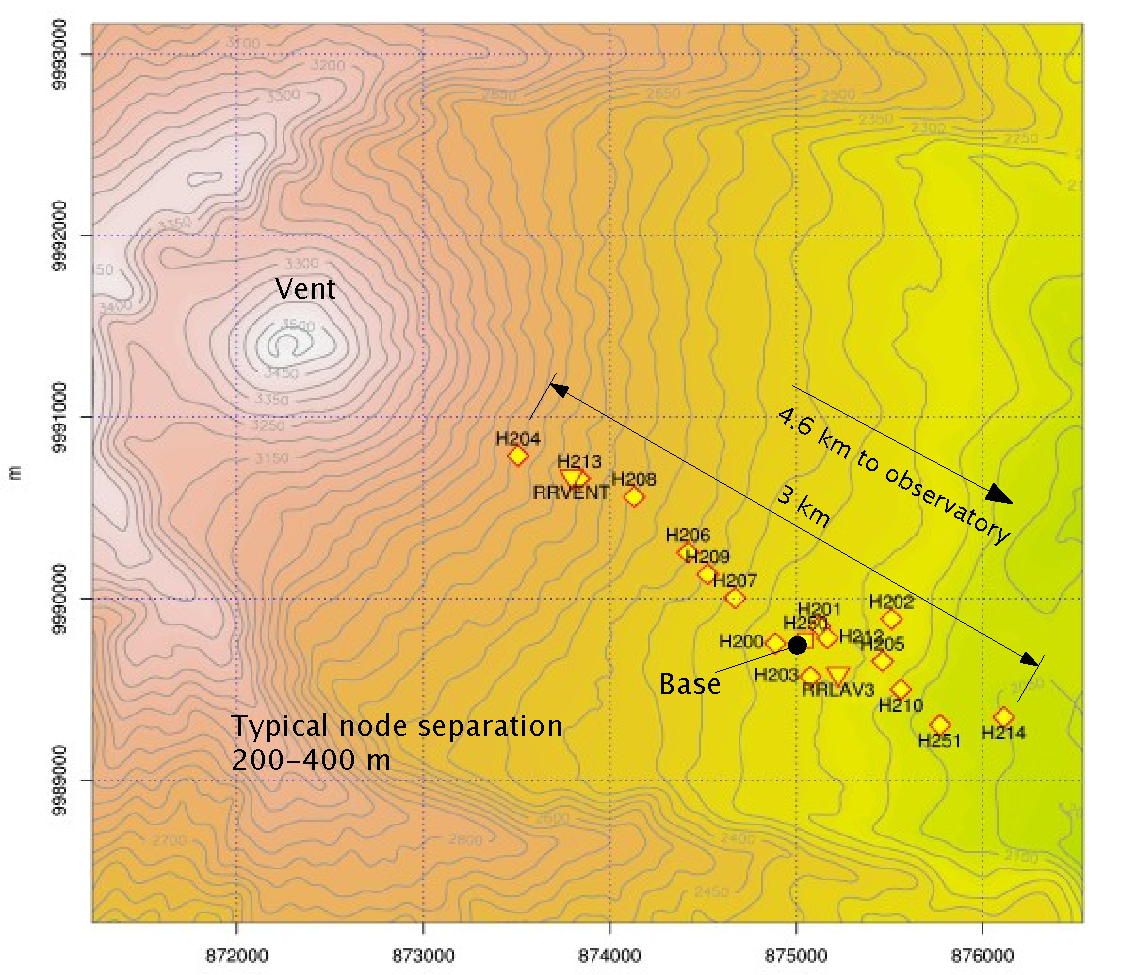
\includegraphics[width=1.0\hsize]{./evaluation/figs/pics/reventador-map.pdf}\\
\textbf{(a)}\\
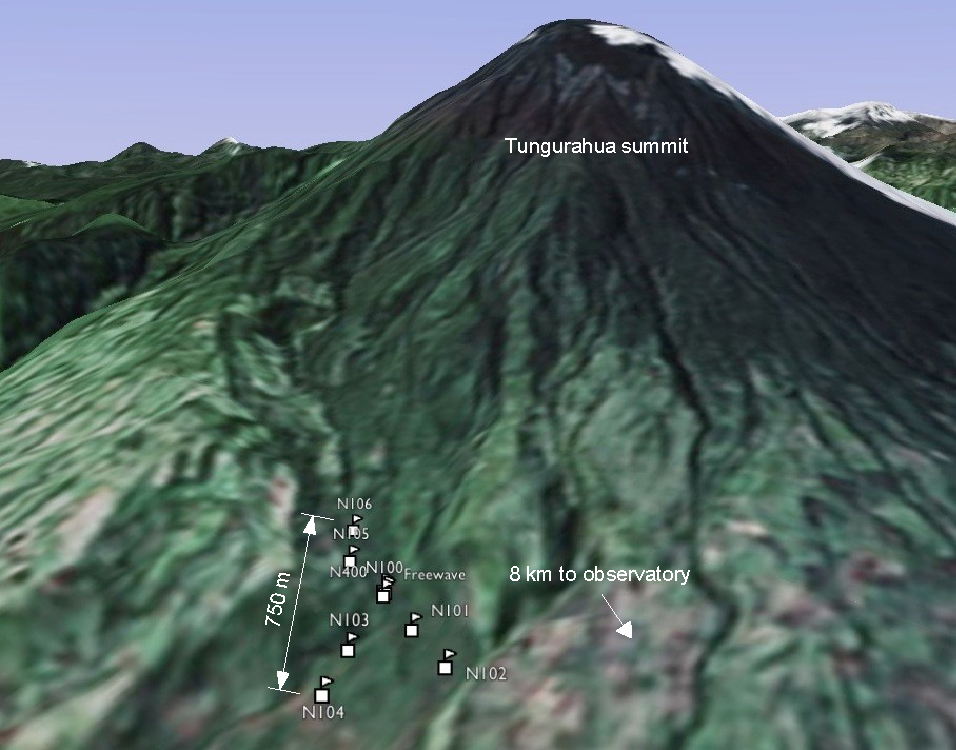
\includegraphics[width=1.0\hsize]{./lance/figs/deploy/deployment-map.pdf}\\
\textbf{(b)}
\end{center}
\caption{{\bf Deployment locations.}
Figures \textbf{a} and \textbf{b} show the locations of our second and third volcano
deployments, in 2005 and 2007. Figure \textbf{a} shows 17 nodes deployed on Reventador
Volcano; \textbf{b} shows eight nodes deployed on Tungurahua Volcano.}
\label{fig-deployment-maps}
\end{figure}


\section{Dissertation Roadmap}

The remainder of the dissertation is organized as follows.

